\begin{minipage}{8cm}
    Un enseignant souhaite décorer sa salle de classe avec une frise chronologique allant de la chute de l’Empire romain (476) à nos jours. Cette frise devra couvrir trois murs de la salle de classe rectangulaire en commençant par le coin nord-ouest et en tournant dans le sens des aiguilles d'une montre. La frise passe au-dessus de la porte et s’étend ainsi sur les murs nord, est et sud.
 \end{minipage}
 \qquad
 \begin{minipage}{8cm}
    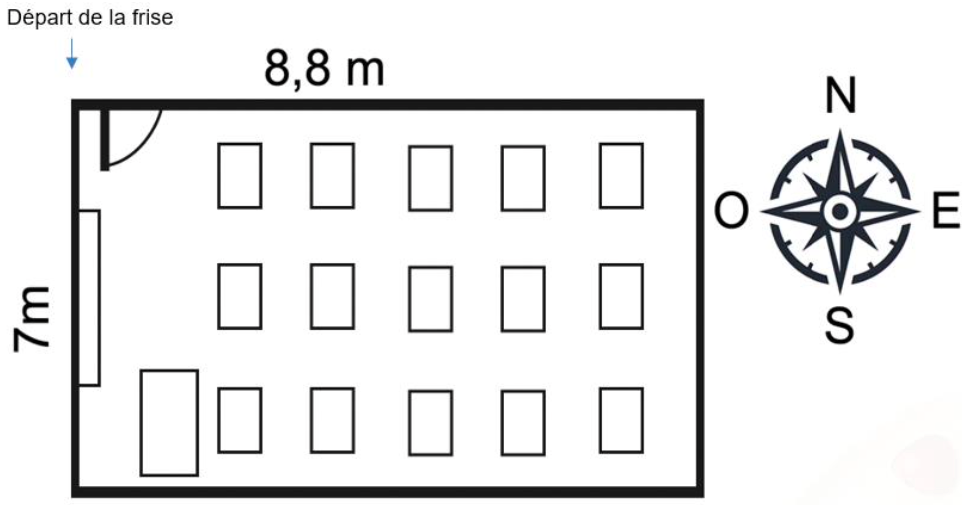
\includegraphics[width=8cm]{Images/Plan}
 \end{minipage}
 \begin{enumerate}
    \setlength{\itemsep}{-1mm}
    \item Pour effectuer cette frise l'enseignant prévoit d'assembler bord à bord des feuilles de format A4 (21 $\times$ 29,7 cm) dans le sens de la longueur. Montrer qu’il faudra 83 feuilles pour réaliser la frise.
    \item Par combien de centimètres est représentée une année sur cette frise chronologique ? Arrondir au millimètre.
    \item L'enseignant a répertorié dans une feuille de calcul automatisé des dates importantes qu'il aimerait faire figurer sur cette frise. \par
       \begin{pspicture}(0.5,0)(16.5,0)
          \psframe[fillstyle=solid,fillcolor=white,linecolor=white](0.515,-3.83)(16.78,-0.14)
       \end{pspicture}
       \footnotesize
       \begin{Tableur}[LargeurUn=8.3cm,Largeur=17mm,Cellule=D2,Colonne=4,Ligne=2,Formule={(C2/29,7)+1}]
          & {\raggedright Année} & {\raggedright Nombre de cm du début de la frise} & \\
          {\raggedright} Fin de l'Antiquité/Début du Moyen-Âge & {\raggedleft 476} & {\raggedleft 0} & \multicolumn{1}{r}{1} \\
          {\raggedright} Fin du Moyen-Âge/Début de l'époque moderne & {\raggedleft 1492} & & \\
          {\raggedright} Fin de l'époque moderne/Début de l'époque contemporaine & {\raggedleft 1789} & & \\
          & & & \\
       \end{Tableur}
       \begin{enumerate}
          \setlength{\itemsep}{-1mm}
          \item Proposer une formule à valider dans la cellule \texttt{C2}, pouvant être étirée vers le bas afin de trouver tous les résultats de la colonne \texttt{C}.
          \item Sachant que la formule validée dans la cellule \texttt{D2} est << \texttt{=ENT(C2/29,7)+1} >>, déterminer à quoi correspondent les nombres de la colonne \texttt{D} au sein de la salle de classe. \newline
             {\it On rappelle que << \texttt{ENT(x)} >> renvoie la partie entière du nombre x.}
       \end{enumerate}
    \item Sur quel mur de la classe se trouvera l’événement << l’accostage de Christophe Colomb sur le continent américain >>, marquant la fin du Moyen-Âge, si on le positionne sur la frise ?
 \end{enumerate}